% =====================================================================
%  Draft 1 Research Paper of This Project
%  E.C.H.O  (Efficient Contextualized History Orchestrator)
%
%  Built on the official IEEE Conference Template (IEEEtran, conference
%  mode, two columns), the same template Overleaf ships as
%  "IEEE Conference Template". Upload this file as main.tex to Overleaf
%  and it compiles with pdfLaTeX without any other files.
%
%  Draft 1 notes for the team:
%   * The paper describes the FINAL intended system, not only the current
%     build. Technical claims were checked against the code in this repo
%     (rse/, enp/, ingestion/, extension/, ste/) on 2026-09-29. Parts that
%     go beyond the current build (to finish before submission):
%       - automatic retry of failed enrichment items (today: manual only,
%         via the ENP_RETRY_FAILED setting)
%       - YouTube revisit rule (the extension must report short revisits)
%   * Results are kept at a high level on purpose. No numbers are claimed.
% =====================================================================
\documentclass[conference]{IEEEtran}
\IEEEoverridecommandlockouts
% The preceding line is only needed to identify funding in the first footnote. If that is unneeded, please comment it out.
\usepackage{cite}
\usepackage{amsmath,amssymb,amsfonts}
\usepackage{algorithmic}
\usepackage{graphicx}
\usepackage{textcomp}
\usepackage{xcolor}
\usepackage{url}
\usepackage{array}
\usepackage{tikz}
\usetikzlibrary{arrows.meta,positioning,fit,calc}
% No automatic hyphens at line ends (style rule for this paper)
\hyphenpenalty=10000
\exhyphenpenalty=10000
\emergencystretch=1.5em
% Author layout: two authors per row, first author flush with the left margin.
% IEEEtran puts a stretchy space before the first author only, which pushed
% the first name to the right. \authorflushleft cancels that space, and
% \linebreakand starts a new row of authors.
\makeatletter
\newcommand{\authorflushleft}{\end{@IEEEauthorhalign}\hskip 0pt plus -1fill\begin{@IEEEauthorhalign}}
\newcommand{\linebreakand}{\end{@IEEEauthorhalign}\par\noindent\mbox{}\begin{@IEEEauthorhalign}}
\makeatother
\def\BibTeX{{\rm B\kern-.05em{\sc i\kern-.025em b}\kern-.08em
    T\kern-.1667em\lower.7ex\hbox{E}\kern-.125emX}}

% Shared style for the two diagrams
\tikzset{
  box/.style={draw, rounded corners=2pt, align=center, font=\footnotesize,
              minimum height=6mm, inner sep=3pt, fill=white},
  store/.style={box, fill=gray!12},
  llm/.style={box, fill=gray!28, font=\footnotesize\bfseries},
  arr/.style={-{Stealth[length=2mm]}, semithick},
  grp/.style={draw, dashed, rounded corners=3pt, inner sep=4pt}
}

\begin{document}

\title{E.C.H.O: An Intent Aware Personal Memory System for Unified Search Across Email, Web, and Video History}

\author{\authorflushleft\IEEEauthorblockN{1\textsuperscript{st} Arjun Sai N}
\IEEEauthorblockA{\textit{Dept. of Computer Science and Engineering} \\
\textit{PES University}\\
Bengaluru, India}
\and
\IEEEauthorblockN{2\textsuperscript{nd} Mohammed Mir Fazlai Ali}
\IEEEauthorblockA{\textit{Dept. of Computer Science and Engineering} \\
\textit{PES University}\\
Bengaluru, India}
\linebreakand
\IEEEauthorblockN{3\textsuperscript{rd} Mohammed Shehzaad Khan}
\IEEEauthorblockA{\textit{Dept. of Computer Science and Engineering} \\
\textit{PES University}\\
Bengaluru, India}
\and
\IEEEauthorblockN{4\textsuperscript{th} Mrigank Jain}
\IEEEauthorblockA{\textit{Dept. of Computer Science and Engineering} \\
\textit{PES University}\\
Bengaluru, India}
\linebreakand
\IEEEauthorblockN{5\textsuperscript{th} Mannuru Shalima Sulthana}
\IEEEauthorblockA{\textit{Dept. of Computer Science and Engineering} \\
\textit{PES University}\\
Bengaluru, India}
}

\maketitle

\begin{abstract}
People read emails, browse web pages, and watch videos every day, but each of these lives in a separate app with its own search box. When someone later wants to find a thing they saw, they often cannot remember where they saw it. This paper presents E.C.H.O, short for Efficient Contextualized History Orchestrator. It is a personal memory system for a single user that brings Gmail, Chrome, and YouTube activity into one searchable store. Every email is kept, but a web page or a video is kept only when simple signals such as time spent, scrolling, and revisits suggest the person paid attention to it. A background worker then cleans each item, places it in a broad category, and turns it into an embedding for meaning based search. Questions are answered by a retrieval graph that makes exactly two calls to a large language model, one to understand the question and one to write the answer. The steps in between use ordinary code and small local models, with no further language model calls. Keyword search and semantic search run side by side, their results are merged by rank, weak results lead to a wider search, and a small local model reorders the final list. The system can also turn a phrase that points to another item, such as a reference to an earlier email, into a fixed point in time. This draft explains the design and the current build. A measured evaluation is planned for a later version.
\end{abstract}

\begin{IEEEkeywords}
personal information management, retrieval augmented generation, hybrid search, reciprocal rank fusion, intent aware capture, local first software
\end{IEEEkeywords}

% ---------------------------------------------------------------------
\section{Introduction}
% ---------------------------------------------------------------------
Think of a student getting ready for a job interview. They receive an email from the company. Over the next few days they read articles about operating systems in Chrome and watch a few tutorials on YouTube. A week later they want to go back to that material. The email is in Gmail, the articles are somewhere in the browser history, and the videos are in the YouTube watch history. Each app has its own search, and none of them knows about the others. The student ends up searching three places, or simply starts over.

The idea of a machine that remembers what a person has seen is old. Bush described it as the memex in 1945 \cite{b1}. Later systems such as Stuff I've Seen \cite{b2} and MyLifeBits \cite{b3} built personal stores of emails, pages, and documents. Two practical problems remain for everyday use today. First, raw history is noisy. The browser records every page that opens, including accidental clicks and pages closed after two seconds. A memory built on that record fills up with things the person never read. Second, a plain search box expects the person to remember exact words. People tend to remember things in a looser way, like ``the OS material I read after the interview email.''

E.C.H.O is our attempt to address both problems. It captures activity from Gmail, Chrome, and YouTube. It keeps a web page or a video only when simple engagement signals show the person paid attention. It stores everything in one data model, enriches each item in the background, and answers questions in natural language. Answers are grounded in the stored items, following the idea of retrieval augmented generation \cite{b4}. Personal data is meant to stay on the user's own machine.

The main contributions of this work are:
\begin{itemize}
\item An intent aware capture layer with separate rules for each source. Emails are always kept, while web pages and videos are kept only when simple signals suggest real attention.
\item A single storage model where emails, pages, and videos share one central table. It is backed by a permanent database, a vector index that can be rebuilt, and a short lived cache.
\item A retrieval graph with a fixed budget of two language model calls. It combines keyword and semantic search through rank fusion, checks result quality with simple rules, widens the search when results are weak, and resolves time references against the user's own items.
\item A privacy first design in which the language model sees only short pieces of text, such as the question, brief excerpts, and item titles, and never the full database. The text of an attachment is shared only when the user asks for it.
\end{itemize}

This is an early draft. We describe the design and the current build, and we keep the discussion of results at a high level. Section~\ref{sec:related} covers related work. Section~\ref{sec:overview} gives an overview of the system. Section~\ref{sec:method} explains capture, storage, enrichment, and retrieval. Section~\ref{sec:privacy} covers privacy. Section~\ref{sec:impl} describes the implementation. Section~\ref{sec:eval} states the expected behavior and the evaluation plan. Section~\ref{sec:limits} lists limitations, and Section~\ref{sec:conc} concludes.

% ---------------------------------------------------------------------
\section{Related Work}\label{sec:related}
% ---------------------------------------------------------------------
\subsection{Personal Information Management}
Bush imagined the memex, a desk that stores a person's books, records, and letters and lets them be found again quickly \cite{b1}. Stuff I've Seen built a single index over information a person had already seen, whether it was an email, a web page, or a document, and used the fact that the person had seen it before as a search cue \cite{b2}. MyLifeBits stored personal information in a SQL database and aimed to store everything that could be captured \cite{b3}. E.C.H.O shares the goal of helping people find things again. It differs in two ways. It filters at capture time, so it does not try to store everything. It also answers questions in natural language instead of offering only a search box.

\subsection{Retrieval Augmented Generation}
Retrieval augmented generation pairs a retriever with a text generator so that answers draw on retrieved documents \cite{b4}. E.C.H.O applies this idea to a personal collection. The retrieval steps are arranged as a fixed graph built with LangGraph \cite{b5}. The language model is used only at the start, to read the question, and at the end, to write the answer.

\subsection{Hybrid Search and Reranking}
Sentence embeddings such as Sentence BERT let us compare texts by meaning using cosine similarity \cite{b6}. E.C.H.O uses a small MiniLM based model \cite{b7} to embed items and the FAISS library \cite{b8} to search the vectors. Keyword search is done with the full text search built into PostgreSQL. The two methods produce scores on very different scales, so adding them directly makes little sense. Reciprocal rank fusion avoids this problem by looking only at the position of each item in each list \cite{b9}. After fusion, a cross encoder reads the question and each candidate together and scores how well they match. Nogueira and Cho showed that this kind of model works well for reranking passages \cite{b10}. The cross encoder in E.C.H.O is a small model trained on the MS MARCO passage ranking data \cite{b11}.

\subsection{Local First Software}
Kleppmann et al.\ describe local first software, where the user keeps ownership of their data and the app works from a copy on their own device \cite{b12}. E.C.H.O follows the same spirit. Its permanent store is designed to run on the user's laptop, and only small, chosen pieces of text are sent to an outside language model.

% ---------------------------------------------------------------------
\section{System Overview}\label{sec:overview}
% ---------------------------------------------------------------------
Fig.~\ref{fig:arch} shows the main parts of E.C.H.O. Three connectors bring in data. The Gmail connector reads email through the Gmail API with OAuth. A Chrome extension watches browsing and YouTube playback in the desktop browser, and the YouTube connector adds video details from the YouTube Data API. All connectors send items through one FastAPI gateway to a storage engine. The storage engine writes each item in a single transaction and skips duplicates.

Data lives in three stores, and each has one job. PostgreSQL is the permanent record of every item. FAISS holds the embedding vectors and can be rebuilt from PostgreSQL at any time. Redis keeps short lived state, such as revisit signals, cached attachment text, and the user's capture settings.

Two parts work on the stored data. The enrichment pipeline runs in the background and prepares new items for search. The retrieval engine answers the user's questions. A React dashboard is the main user interface. A wellbeing module that describes time patterns without judging them is also part of the wider design. It is still being validated, so this draft leaves it out of scope.

\begin{figure}[t]
\centering
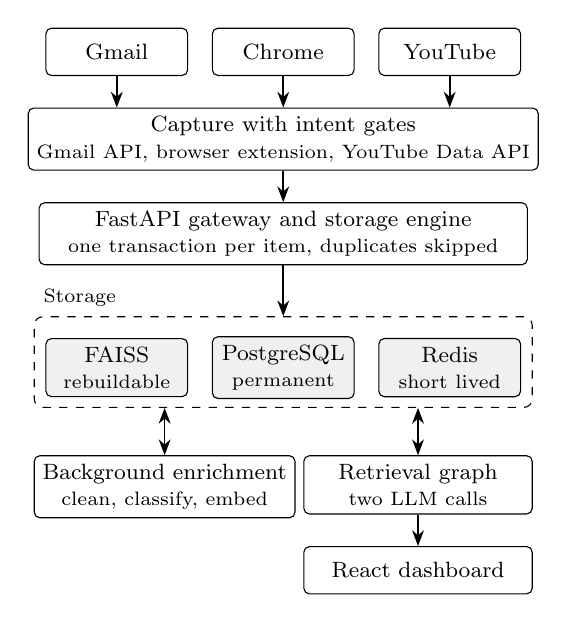
\begin{tikzpicture}[node distance=4mm and 3mm]
  \node[box, minimum width=18mm] (gm) {Gmail};
  \node[box, minimum width=18mm, right=of gm] (ch) {Chrome};
  \node[box, minimum width=18mm, right=of ch] (yt) {YouTube};
  \node[box, minimum width=62mm, below=of ch] (cap)
      {Capture with intent gates\\ \scriptsize Gmail API, browser extension, YouTube Data API};
  \node[box, minimum width=62mm, below=of cap] (gw)
      {FastAPI gateway and storage engine\\ \scriptsize one transaction per item, duplicates skipped};
  \node[store, minimum width=18mm, below=9mm of gw] (pg) {PostgreSQL\\ \scriptsize permanent};
  \node[store, minimum width=18mm, left=of pg] (fa) {FAISS\\ \scriptsize rebuildable};
  \node[store, minimum width=18mm, right=of pg] (rd) {Redis\\ \scriptsize short lived};
  \node[grp, fit=(fa)(pg)(rd), inner ysep=5pt, yshift=2pt] (st) {};
  \node[font=\scriptsize, anchor=south west] at (st.north west) {Storage};
  \node[box, minimum width=29mm, below=6mm of st.south west, anchor=north west] (enp)
      {Background enrichment\\ \scriptsize clean, classify, embed};
  \node[box, minimum width=29mm, below=6mm of st.south east, anchor=north east] (rse)
      {Retrieval graph\\ \scriptsize two LLM calls};
  \node[box, minimum width=29mm, below=of rse] (ui) {React dashboard};
  \draw[arr] (gm) -- (gm |- cap.north);
  \draw[arr] (ch) -- (cap);
  \draw[arr] (yt) -- (yt |- cap.north);
  \draw[arr] (cap) -- (gw);
  \draw[arr] (gw) -- (st.north);
  \draw[arr, {Stealth[length=2mm]}-{Stealth[length=2mm]}] (enp.north) -- (enp.north |- st.south);
  \draw[arr, {Stealth[length=2mm]}-{Stealth[length=2mm]}] (rse.north) -- (rse.north |- st.south);
  \draw[arr] (rse) -- (ui);
\end{tikzpicture}
\caption{Main parts of E.C.H.O. PostgreSQL is the permanent record. FAISS can be rebuilt from it, and Redis holds short lived state and the capture settings.}
\label{fig:arch}
\end{figure}

% ---------------------------------------------------------------------
\section{Methodology}\label{sec:method}
% ---------------------------------------------------------------------
\subsection{Intent Aware Capture}
Each source has its own rule for deciding what to keep. Table~\ref{tab:gates} lists the current rules. The numbers are starting values and we expect to tune them.

Gmail is treated differently from the other two sources. Every received email is saved when it arrives, whether or not it is opened. Emails come to the user rather than being chosen by them, the daily volume is small, and even an unread email may matter later. When the user opens an email in Gmail on the web, the extension records reading time for it.

For Chrome, the extension uses a two phase gate. In the first phase the page must stay in the foreground for a few seconds. Pages that fail this phase are dropped right away. In the second phase at least one sign of attention must be present. This can be enough foreground time, enough scrolling, a click or text selection on the page, or a visit to the same page within the past 24 hours. Time counts only when the tab is active, the browser window has focus, and the user has not been idle for 30 seconds. Revisits are remembered in Redis for 24 hours. A page that passes the first phase and was also seen in that window is kept, even if the user did not scroll or click.

For YouTube, a video is kept if it plays in the foreground long enough, if at least half of it is watched, if the user pauses, seeks, or changes the playback speed, or if the same video was opened within the past 24 hours. The last rule means a video the user keeps coming back to is kept even when no single visit was long. Shorts are detected from the page address and have a slightly lower time bar.

\begin{table}[t]
\caption{Current Capture Rules for Each Source}
\label{tab:gates}
\centering
\renewcommand{\arraystretch}{1.15}
\begin{tabular}{|>{\raggedright\arraybackslash}p{1.35cm}|>{\raggedright\arraybackslash}p{6.2cm}|}
\hline
\textbf{Source} & \textbf{An item is kept when} \\
\hline
Gmail & Always, at arrival. Reading time is added when the email is opened. \\
\hline
Chrome & Phase 1: at least 5~s in the foreground. Phase 2: any one of at least 10~s in the foreground, at least 25\% scroll depth, one click or text selection, or a revisit within 24~hours. \\
\hline
YouTube & Any one of at least 20~s of foreground playback (15~s for Shorts), at least half of the video watched, a pause, seek, or change of playback speed, or a revisit within 24~hours. \\
\hline
\end{tabular}
\end{table}

\subsection{Storage Model}
Every email, page, and video becomes one row in a central table of memory items. Details that belong to only one source go into a matching source table for Gmail, Chrome, or YouTube. Engagement data, such as reading time, watch time, and revisit counts, lives in its own table because it changes often. The full schema has 16 tables.

A uniqueness rule on the pair of source type and source id stops the same item from being saved twice, for example when a connector restarts. Deletion is soft, so a deleted item is hidden from every query. Items are first saved in a raw state and marked as not yet processed. This keeps the capture path fast and safe if the system crashes.

\subsection{Background Enrichment}
A background worker picks up items that are not yet processed. It never runs on the capture path, so slow enrichment does not slow down capture. For each item it does four things.

\textit{Cleaning.} Emails lose their HTML, tracking pixels, signatures, and quoted replies. For a reply email, keywords from earlier emails in the same thread are added, so a short ``Re:'' message can still be found by its topic. Web pages go through a readability step that keeps the main article text and drops menus, ads, and footers. Videos use the title, description, channel name, and the transcript when one is available.

\textit{Embedding.} The cleaned text is turned into a 384 dimension vector using the \texttt{all-MiniLM-L6-v2} sentence model \cite{b6}, \cite{b7}. The vector is added to the FAISS index without rebuilding the whole index.

\textit{Classification.} Each item is placed into one of five broad groups: work, study, entertainment, personal, or misc. A four stage cascade does this. Stage one uses structural signals from the source, such as Gmail category labels, academic email domains, or the YouTube video category. Stage two looks up the web domain in a fixed table. Stage three compares the item's embedding with a center point for each group and accepts the answer only if the best match is clear enough and well ahead of the second best. Stage four asks the language model for a single label, and it is reached only by items the first three stages could not place. An item always gets a group, and misc is the fallback.

\textit{State tracking.} Each item is marked as processed or failed. Failed items are kept apart and retried automatically, so they are never counted as done by mistake and are not lost.

Email attachments are handled in two tiers. At capture time only the file name, type, and size are stored. The full text is extracted later, only when a question needs it, as described below. The extracted text is cached in Redis for one hour, and the file itself is never stored.

\subsection{Retrieval Graph}
Questions are answered by a fixed graph, shown in Fig.~\ref{fig:graph}. The language model is called exactly twice per question, no matter how many times the search loops. Everything between the two calls is ordinary Python code plus two small local models, one for embeddings and one for reranking. This makes each step easy to inspect and test.

\begin{figure}[t]
\centering
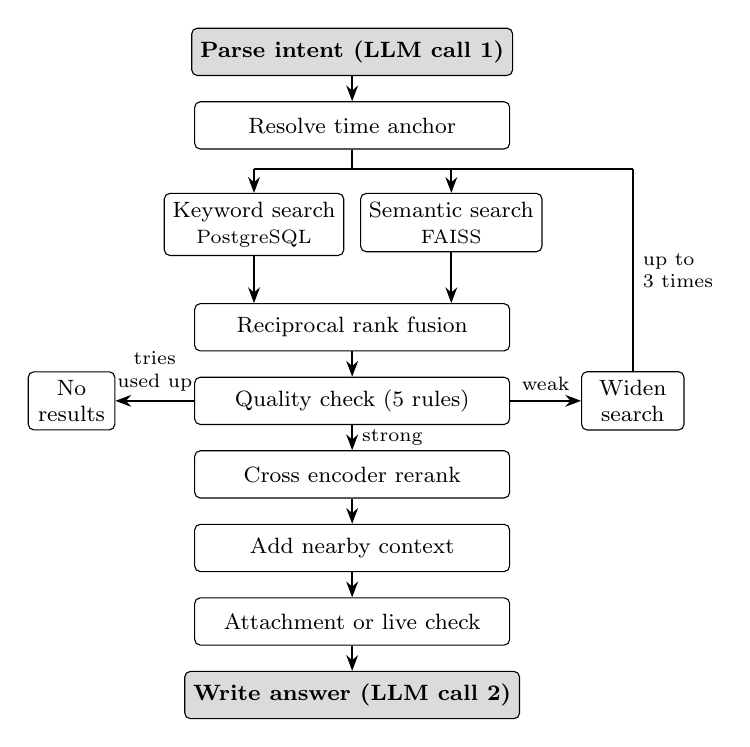
\begin{tikzpicture}[node distance=3.2mm and 3mm]
  \node[llm, minimum width=40mm] (pi) {Parse intent (LLM call 1)};
  \node[box, minimum width=40mm, below=of pi] (ta) {Resolve time anchor};
  \coordinate (bus) at ($(ta.south)+(0,-2.5mm)$);
  \node[box, minimum width=19mm, anchor=north east] (kw) at ($(bus)+(-1mm,-3mm)$) {Keyword search\\ \scriptsize PostgreSQL};
  \node[box, minimum width=19mm, anchor=north west] (se) at ($(bus)+(1mm,-3mm)$) {Semantic search\\ \scriptsize FAISS};
  \node[box, minimum width=40mm, anchor=north] (rrf) at ($(bus)+(0,-17mm)$) {Reciprocal rank fusion};
  \node[box, minimum width=40mm, below=of rrf] (qc) {Quality check (5 rules)};
  \node[box, minimum width=13mm, right=9mm of qc] (wd) {Widen\\search};
  \node[box, minimum width=11mm, left=10mm of qc] (nr) {No\\results};
  \node[box, minimum width=40mm, below=of qc] (ce) {Cross encoder rerank};
  \node[box, minimum width=40mm, below=of ce] (nb) {Add nearby context};
  \node[box, minimum width=40mm, below=of nb] (at) {Attachment or live check};
  \node[llm, minimum width=40mm, below=of at] (sy) {Write answer (LLM call 2)};
  \draw[arr] (pi) -- (ta);
  \draw[semithick] (ta.south) -- (bus);
  \draw[semithick] (bus -| kw.center) -- (bus -| wd.center);
  \draw[arr] (bus -| kw.center) -- (kw.north);
  \draw[arr] (bus -| se.center) -- (se.north);
  \draw[semithick] (wd.north) -- node[right, font=\scriptsize, align=left] {up to\\3 times} (wd.north |- bus);
  \draw[arr] (kw.south) -- (kw.south |- rrf.north);
  \draw[arr] (se.south) -- (se.south |- rrf.north);
  \draw[arr] (rrf) -- (qc);
  \draw[arr] (qc) -- node[above, font=\scriptsize] {weak} (wd);
  \draw[arr] (qc) -- node[above, font=\scriptsize, align=center] {tries\\used up} (nr);
  \draw[arr] (qc) -- node[right, font=\scriptsize] {strong} (ce);
  \draw[arr] (ce) -- (nb);
  \draw[arr] (nb) -- (at);
  \draw[arr] (at) -- (sy);
\end{tikzpicture}
\caption{The retrieval graph. Shaded boxes are the only two language model calls. When the search is widened, both search branches run again.}
\label{fig:graph}
\end{figure}

\textit{Parse intent.} The first call reads the question together with the conversation so far. It returns a structured JSON object. The object lists the sources to search, any time filter, a cleaned query, a few alternative phrasings of the query, and flags that say whether an attachment or live data is needed. It also captures time anchors. For a question such as ``OS material after the interview email,'' it records the anchor ``interview email'' and the relation ``after.''

\textit{Resolve time anchor.} The anchor is looked up among the user's own items, first by keyword and then by meaning if needed. The time of the matching item becomes a hard limit that both search branches must obey. If no anchor item is found, the search runs without the limit.

\textit{Parallel search.} The keyword branch uses PostgreSQL full text search over titles, text, senders, domains, and channel names. The semantic branch embeds each phrasing of the query and searches FAISS. Because the stored vectors are not normalized, cosine similarity is computed directly from the vectors instead of reading it from the index distances. The two branches run in the same step of the graph.

\textit{Fusion.} The two ranked lists are merged with reciprocal rank fusion \cite{b9}. For an item $d$, the fused score is
\begin{equation}
\mathrm{RRF}(d) = \sum_{b \in B} \frac{1}{k + r_b(d)}, \label{eq:rrf}
\end{equation}
where $B$ is the set of branches that returned $d$, $r_b(d)$ is its position in branch $b$ starting from 1, and $k = 60$. Only positions are used, so the two score scales never need to be matched. The top 50 fused items move on.

\textit{Quality check and widening.} Five simple rules decide whether the results are strong. The results are weak or empty if there are none, if none come from a source the user asked for, if none fall inside the time window, if there are fewer than two, or if the best cosine similarity is below 0.35. Weak results trigger a wider search, and the graph runs both branches again. Each attempt relaxes one more thing. The first attempt stretches the time window, opens all sources, or shortens the query. The second removes the time filters and the anchor. The third drops keyword matching and all filters, and searches a larger part of the vector index. After three attempts the graph returns a clear no results message.

\textit{Reranking.} A local cross encoder \cite{b10}, \cite{b11} scores each remaining item against the original question. The final score mixes this with an effort score:
\begin{equation}
s(d) = 0.8\,\sigma\big(c(q,d)\big) + 0.2\,e(d), \label{eq:final}
\end{equation}
where $c(q,d)$ is the cross encoder output for question $q$ and item $d$, $\sigma$ is the sigmoid function, and $e(d)$ is the effort score between 0 and 1. The effort score is the average of the engagement signals available for the item, such as reading or watch time, scroll depth, revisits, interactions, and how much of a video was watched. It rewards items the user spent real attention on. By design, the score has no term for how recent an item is.

\textit{Nearby context.} For the top three items, the graph adds close neighbors. For an email these are other emails in the same thread. For a page or a video these are items from the same browsing session or from within five minutes of it.

\textit{Attachments and live data.} If the question asks for the content of a file and one of the top three results is an email with attachments, the attachments of the first such email are downloaded through the Gmail API. Text is extracted only from files that are small or whose names match the question, and the amount of text kept is capped. If the question asks about something that just arrived, the graph polls Gmail once and loads the newest items.

\textit{Write answer.} The second call receives the question, the conversation so far, and the top ten results. Each result is passed as a short excerpt of at most 500 characters along with its title, source, time, and the sender, website, or channel it came from. Titles of nearby items are added as context. The model writes an answer that cites its sources. If the language model call fails, the system still returns a simple list of the ranked results.

\subsection{Conversation Memory}
Each conversation has a session id, and every turn is saved in PostgreSQL. Both language model calls see the history of the current session. This lets a follow up question such as ``show me Chrome pages about that topic after that email'' refer back to an earlier answer.

% ---------------------------------------------------------------------
\section{Privacy by Design}\label{sec:privacy}
% ---------------------------------------------------------------------
Privacy shapes several decisions in E.C.H.O. Nothing from incognito tabs is ever captured. It does not record typed text or form input. For work apps such as Slack, Notion, and Jira, it never reads page content. Passwords and credentials are never touched, and OAuth tokens are stored encrypted.

The language model sees only what it needs. The first call gets the question and the conversation history. The second call gets the question, the history, and for each top result a short excerpt, its title, its time, and its sender, website, or channel. Full email bodies, full pages, transcripts, database rows, and vectors are never sent. Any other text the model sees is small and has a fixed limit. When the user explicitly asks for the content of an attachment, the extracted text of that email's attachments is included, up to a few thousand characters. The background classifier asks the model for help only with items it cannot place on its own, and even then it sends just the title and a short excerpt of about 300 characters.

The user also has direct control. Each source can be turned off, and specific domains and senders can be excluded. Items can be deleted, and all data can be exported as JSON or CSV.

% ---------------------------------------------------------------------
\section{Implementation}\label{sec:impl}
% ---------------------------------------------------------------------
Table~\ref{tab:stack} summarizes the technology used. The backend is written in Python and served with FastAPI. The retrieval graph is built with LangGraph \cite{b5}. Language model access goes through LangChain wrappers, so switching between hosted providers or a locally run model is a change to one configuration entry. Embeddings and the cross encoder run locally through the sentence transformers library. The dashboard is written in React with TypeScript. The browser extension uses Chrome Manifest V3.

In the final setup, PostgreSQL runs on the user's laptop. During development the team uses a hosted PostgreSQL instance so that all members can work against the same schema.

\begin{table}[t]
\caption{Technology Used in the Current Build}
\label{tab:stack}
\centering
\renewcommand{\arraystretch}{1.15}
\begin{tabular}{|>{\raggedright\arraybackslash}p{2.0cm}|>{\raggedright\arraybackslash}p{5.55cm}|}
\hline
\textbf{Layer} & \textbf{Technology} \\
\hline
Capture & Chrome extension (Manifest V3), Gmail API, YouTube Data API \\
\hline
Backend & Python, FastAPI \\
\hline
Storage & PostgreSQL, FAISS, Redis \\
\hline
Enrichment & Readability extraction, PDF and DOCX text extraction \\
\hline
Models & \texttt{all-MiniLM-L6-v2} embeddings, \texttt{ms-marco-MiniLM-L-6-v2} cross encoder, a configurable LLM \\
\hline
Retrieval & LangGraph, LangChain \\
\hline
Interface & React, TypeScript, Vite \\
\hline
\end{tabular}
\end{table}

% ---------------------------------------------------------------------
\section{Expected Behavior and Evaluation Plan}\label{sec:eval}
% ---------------------------------------------------------------------
This draft does not report measured results. Here we describe, at a high level, what a user can expect from the system, and how we plan to measure it.

\subsection{Expected Behavior}
In general, a user types a question in plain language and gets back a short written answer along with the items it was based on. Those items can come from more than one source. A question tied to an event, such as material read after a given email, is handled by finding that event first and then searching around it. A follow up question can refer to something from an earlier turn. Accidental page opens and very short video views should not show up in answers, because they are not captured in the first place. If the language model cannot be reached, the user still gets a list of matching items instead of an error.

\subsection{Evaluation Plan}
We plan to evaluate E.C.H.O along four lines.
\begin{itemize}
\item \textit{Retrieval quality.} Build a set of test questions with known relevant items, and compare the hybrid graph against keyword only and semantic only search.
\item \textit{Coverage across sources.} Check how often answers correctly draw on items from more than one source when the question calls for it.
\item \textit{Response time.} Measure the time for a full question, with and without attachment extraction.
\item \textit{Capture accuracy and privacy.} Replay scripted browsing and viewing sessions to check the intent gates, and audit every outbound call to confirm that only the allowed text leaves the machine.
\end{itemize}

% ---------------------------------------------------------------------
\section{Limitations and Future Work}\label{sec:limits}
% ---------------------------------------------------------------------
E.C.H.O has clear limits at this stage. It has been built for desktop Chrome, so mobile apps are not covered. YouTube history starts from the day the extension is installed, and background or picture in picture playback is not tracked. Text extraction from image attachments needs an extra OCR tool and is optional. Periodic jobs, such as refreshing the classifier's group centers, are run by hand for now. The two language model calls depend on the limits of whichever provider is configured. Finally, the wellbeing module is built in an initial form but has not been validated on real data yet.

Future work will focus on the evaluation described above, tuning the capture rules and retrieval settings based on what we measure, and bringing the wellbeing module into scope.

% ---------------------------------------------------------------------
\section{Conclusion}\label{sec:conc}
% ---------------------------------------------------------------------
E.C.H.O brings email, browsing, and video history into one personal memory that a user can search in plain language. It keeps all emails but only the pages and videos the user paid attention to, stores them in one data model, and prepares them for search in the background. Questions are answered by a fixed retrieval graph that calls a language model only twice per question and handles every other step with testable code and small local models. This draft sets out the design and the current build. The next version will add measured results.

\section*{Acknowledgment}
We thank the Department of Computer Science and Engineering, PES University, for its support during this capstone project.

% Balances the two columns on the last page. Adjust the number if the reference list changes.
\IEEEtriggeratref{8}
\begin{thebibliography}{00}
\bibitem{b1} V. Bush, ``As we may think,'' \textit{The Atlantic Monthly}, vol. 176, no. 1, pp. 101--108, Jul. 1945.
\bibitem{b2} S. Dumais, E. Cutrell, J. J. Cadiz, G. Jancke, R. Sarin, and D. C. Robbins, ``Stuff I've seen: A system for personal information retrieval and re-use,'' in \textit{Proc. 26th Annu. Int. ACM SIGIR Conf. Research and Development in Information Retrieval}, Toronto, Canada, 2003, pp. 72--79.
\bibitem{b3} J. Gemmell, G. Bell, and R. Lueder, ``MyLifeBits: A personal database for everything,'' \textit{Commun. ACM}, vol. 49, no. 1, pp. 88--95, Jan. 2006.
\bibitem{b4} P. Lewis, E. Perez, A. Piktus, F. Petroni, V. Karpukhin, N. Goyal, H. K\"{u}ttler, M. Lewis, W. Yih, T. Rockt\"{a}schel, S. Riedel, and D. Kiela, ``Retrieval-augmented generation for knowledge-intensive NLP tasks,'' in \textit{Advances in Neural Information Processing Systems}, vol. 33, 2020, pp. 9459--9474.
\bibitem{b5} LangChain, ``LangGraph,'' GitHub repository. [Online]. Available: \url{https://github.com/langchain-ai/langgraph} (accessed Sep. 29, 2026).
\bibitem{b6} N. Reimers and I. Gurevych, ``Sentence-BERT: Sentence embeddings using Siamese BERT-networks,'' in \textit{Proc. 2019 Conf. Empirical Methods in Natural Language Processing and 9th Int. Joint Conf. Natural Language Processing (EMNLP-IJCNLP)}, Hong Kong, China, 2019, pp. 3982--3992.
\bibitem{b7} W. Wang, F. Wei, L. Dong, H. Bao, N. Yang, and M. Zhou, ``MiniLM: Deep self-attention distillation for task-agnostic compression of pre-trained transformers,'' in \textit{Advances in Neural Information Processing Systems}, vol. 33, 2020, pp. 5776--5788.
\bibitem{b8} J. Johnson, M. Douze, and H. J\'{e}gou, ``Billion-scale similarity search with GPUs,'' \textit{IEEE Trans. Big Data}, vol. 7, no. 3, pp. 535--547, Jul. 2021.
\bibitem{b9} G. V. Cormack, C. L. A. Clarke, and S. B\"{u}ttcher, ``Reciprocal rank fusion outperforms Condorcet and individual rank learning methods,'' in \textit{Proc. 32nd Int. ACM SIGIR Conf. Research and Development in Information Retrieval}, Boston, MA, USA, 2009, pp. 758--759.
\bibitem{b10} R. Nogueira and K. Cho, ``Passage re-ranking with BERT,'' arXiv:1901.04085, 2019.
\bibitem{b11} P. Bajaj \textit{et al.}, ``MS MARCO: A human generated machine reading comprehension dataset,'' arXiv:1611.09268, 2016.
\bibitem{b12} M. Kleppmann, A. Wiggins, P. van Hardenberg, and M. McGranaghan, ``Local-first software: You own your data, in spite of the cloud,'' in \textit{Proc. ACM SIGPLAN Int. Symp. New Ideas, New Paradigms, and Reflections on Programming and Software (Onward!)}, 2019, pp. 154--178.
\end{thebibliography}

\end{document}
